\documentclass[10pt,twocolumn]{article} 

% use the oxycomps style file
\usepackage{oxycomps}

% read references.bib for the bibtex data
\bibliography{references}

% include metadata in the generated pdf file
\pdfinfo{
    /Title (Comps Proposal Paper)
    /Author (Sammy Sanchez)
}

% set the title and author information
\title{CS COMPS Proposal Paper}
\author{Sammy Sanchez}
\affiliation{Occidental College}
\email{sanchezs@oxy.edu}

\begin{document}

\maketitle

\section{Problem Context}

For the project that I am doing, I want to make it easier for people that look at sports statistics to visualize the data on graphs to evaluate players. This will be a website or web app that can help people analyze sports players for fantasy sports that helps them pick the best player of their choice for their chosen stats. The user would be able to pick and group stats of the sport they are playing fantasy in and pick a player the want to compare those stats to. A scatter graph will be created to show where the player's data is at and if other players have similar stats. The stats used for the graph will also be in a chart below the graph to see the data. The user would be able to visualize and evaluate the players that are similar to the chosen player and decide on if they would use the player in fantasy sports for their team. The way the user picks that stats will also have a description of how the stat chosen is calculated to give more detail because a person might not know how it is calculated and what is used to calculate it. An example would be True Shooting stat in basketball and would read "TS\% stands for True shooting percentage and it is a measure of shooting efficiency that takes into account field goals, 3-point field goals, and free throws". It will also help users that are interested in sports analytics because of how the app will be a unique way of combining stats to visualize a spectrum of where players line up against each other. It will also be different compared to other databases because of the ability to include stats like body height, weight and age to evaluate players. 

There are no fantasy sports apps that analyzes stats that the users pick specifically and displays it on a graph. Fantasy apps currently only display stats on data charts which makes it hard to virtually analyze stats. Being able to visualize stats and players with specific stats chosen will help any fantasy team owner when picking players for their team. The help will come when a fantasy team owner wants to get a player that is similar to another player statistically and it will help generate points for the team over the season. When the best players are chosen by other teams, it gets harder to find players that produce the same amount of fantasy points and this will help target stats that produce points. Being able to group important stats together will help the owner to see how good other players are to a player that does well in the sport. The graph will show a correlation of the stats picked for evaluation, and it will help drive a decision of what player to pick for the team. 

My project would be useful for fantasy players because it will give them an understanding of how different NBA players can be similar statistically which can help a fantasy team accumulate points over the season. It is helpful when the so called "super stars" are picked in the first couple rounds of a fantasy draft and that there are other players available that have similar statistics to those stars which can help make a positive impact on your team. The impact this project would have on positive players is how they view these NBA players based on what stats they want to compare and teach them about impact players that are not considered stars. 


\section{Technical Background}


For my approach of doing this project, I need to learn how to create a website that can query data from sports stats websites like Sports Reference created by Sean \textcite{sportsReference} and ESPN created by Bill \textcite{espn}. When querying the data it will allow the user to gather those stats from the database websites and create a graph based on the chosen stats. I would have to learn how to create graphs from the gathered data using Python or another coding language that can create graphs. I would need to use an algorithm that can group stats together and make plots on a graph that uses the stats for each player that is being compared. The mathematical equations used would have to be programmed to be implemented when creating the graph based on that stats chosen and might require an algorithm to do it. When the mouse is over the data point, it would have to be programmed to show the player's name on the point. Below the graph would also show the stats used in a chart with other players names. This could be done with querying to select stats from the sports statistic websites and display them on a chart generated from the query. For selecting stats and the player, I would have to program the website to have drop down lists that display all the possible options to choose from.

The way people perceived sports data/statistics over the years has changed drastically because of how reliable sports stats have become for professional teams. In an article written by Alyssa \textcite{sportsStats}, she discusses how sports stats were not used as heavily going back to the 1980's and 90's because of subjective gut feelings about players. These were usually biased because of how a coach or front office person would feel about that player. In 2002, she discussed how the Oakland Athletic in the MLB used statistical analysis to created a baseball team of lesser-known players to have a great season and make the playoffs and many people frowned upon the idea of using statistical analysis to make a team that way. Now, sports statics analysis has taken over how fans and employees of these professional teams views players and evaluate them. Many companies have made their own algorithms to track almost all aspects of a respective sport and evaluate the data that they keep track of. 

Another way people have used sports statistics is to predict MVP awards using algorithms and machine learning. In an article written by David \textcite{MVPpredict}, he discusses the way the NBA MVP is awarded based on the people the vote for it and how an AI can predict who is going to win it. The algorithm compares historical data of past MVP winners through two different equations and sees how accurately the AI predicts the MVP. It used MAE (Mean Absolute Error) and R² (coefficient of determination) to evaluate the the MVP as seen in Figure 1. The experiments that were used was to see if it correctly identified the MVP for a specific year and would calculate the accuracy of guessing the MVP correctly. 

\begin{figure}
    \centering
    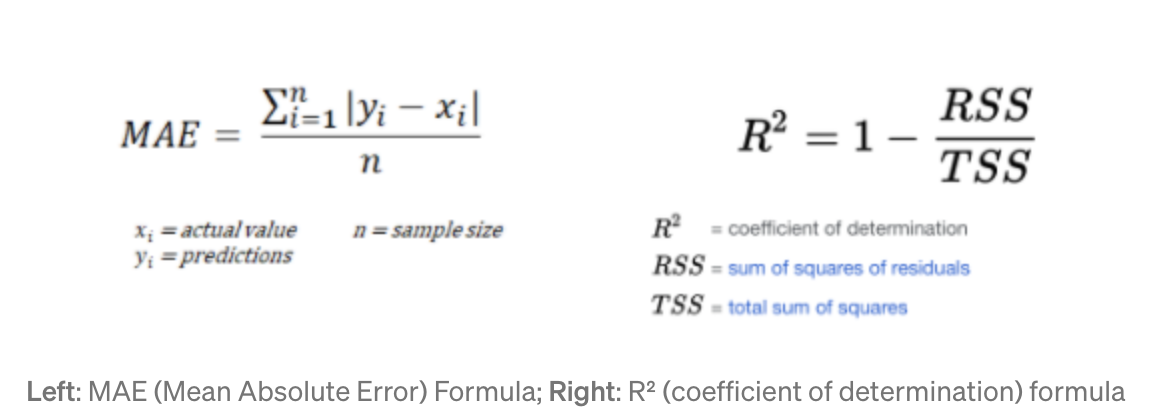
\includegraphics[width=.95\linewidth]{stats.png}
    \caption{
        MAE and R²
    }
    \label{fig:second-page-1}
\end{figure}


\section{Prior Work}

The prior work that has been done is a website called "NBA Player Performance and Scouting Explorer" and the website is created by \textcite{dash}.
It is designed to be used as a way to view and group NBA players with stats on graphs. One of the graphs uses body weight and height as a way to group players with higher physicality or you can group the player strictly off statistics. The players are grouped in the graph based on their position in basketball and a player is selected to be compared to with a chart listed below the graph with the stats. It allows the user to also group players based on the custom stats they choose to evaluate players. Another option to use in this app is how stats picked are grouped together and groups are made for players that are similar with those stats. It is something similar with what I want to do with my project, but in this app, the stats that can be used are limited and I want to expand it with more. It is also only used for basketball players and I would expand it to other sports like baseball and football. In Figure 2, it shows the visualization of Steph Curry compared to other players in the NBA that have a similar physicality to him, but also shows how statistical data compared to him as well. The inspiration for this website can be to find good NBA players and be unbiased using their app. As a user, they can pick their favorite player and compare them to other players using stats or physicality of the chosen player and the results will be unbiased. Biases in sports are very common because of many factors like home team, not liking a player because of their persona and etc.

\begin{figure}
    \centering
    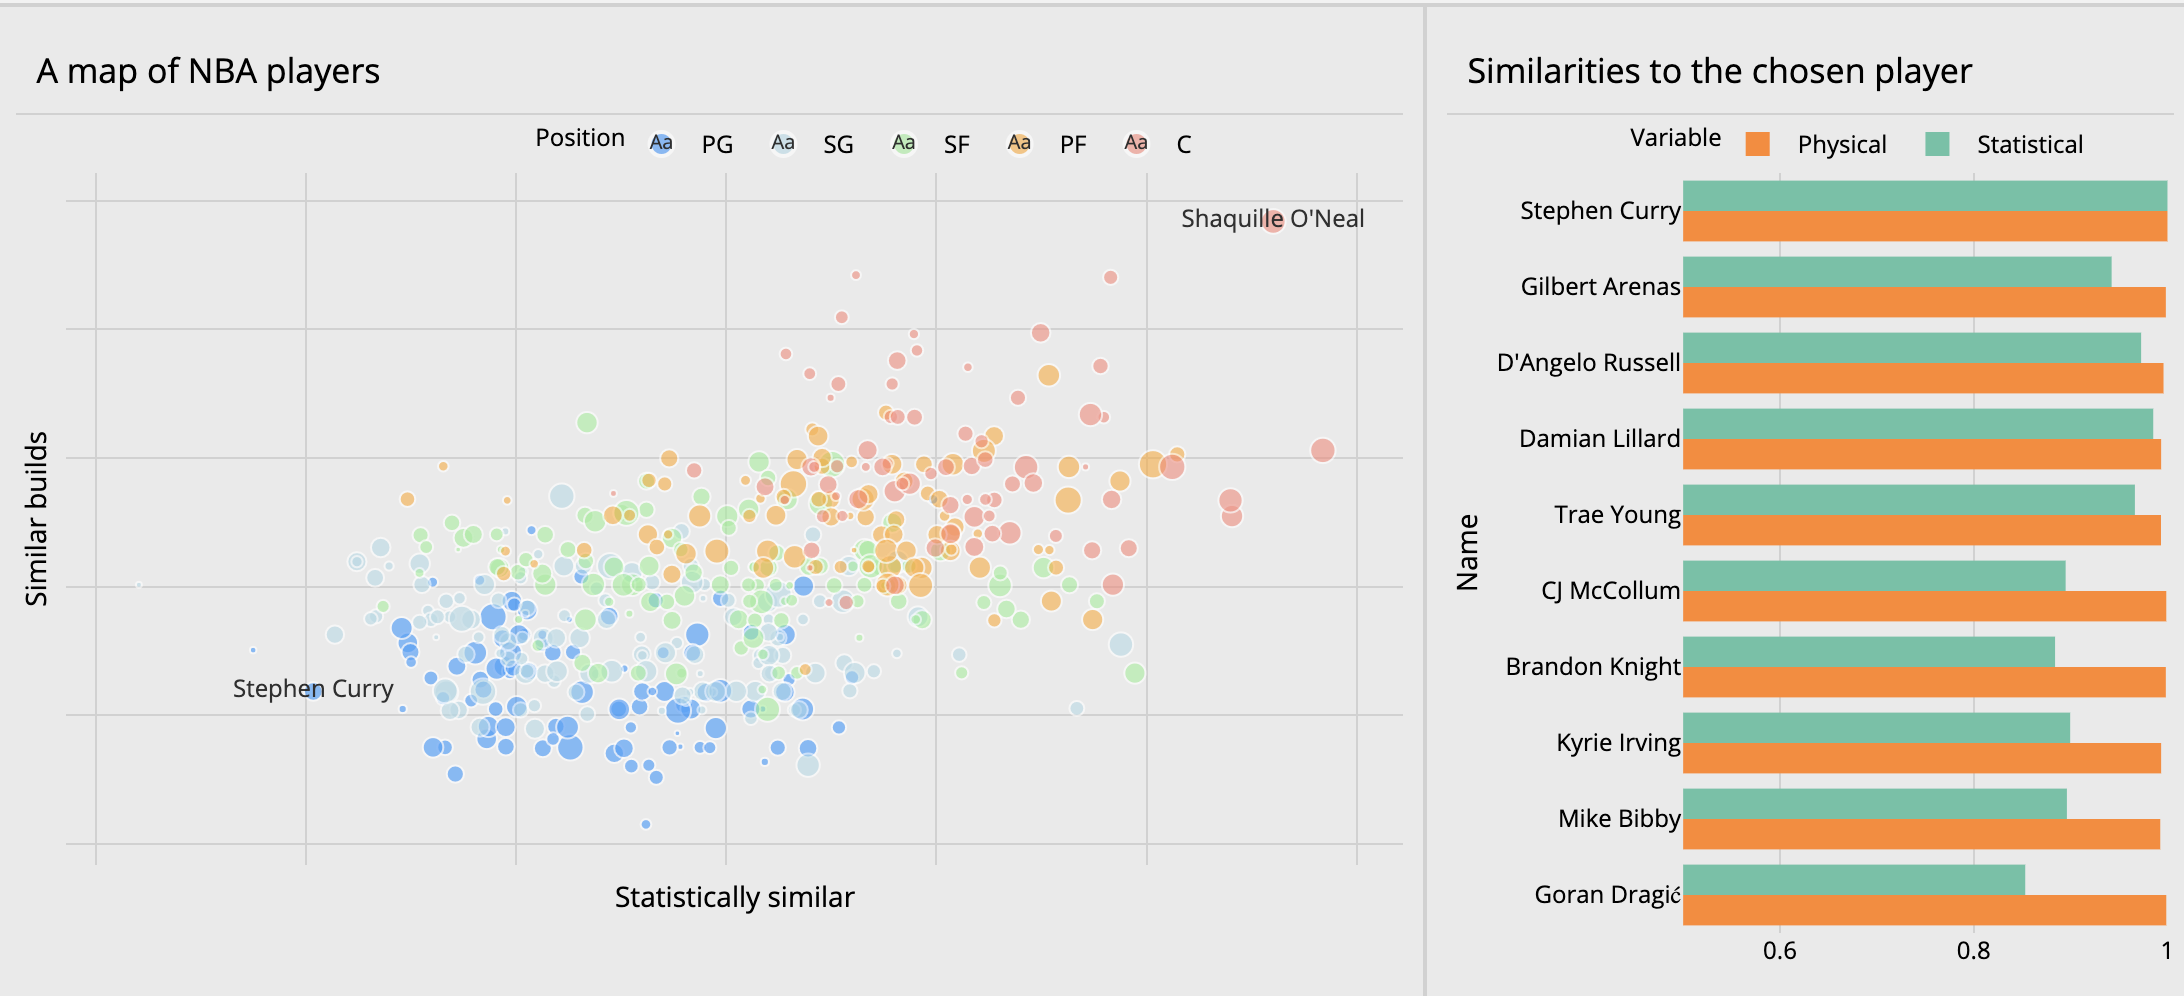
\includegraphics[width=.98\linewidth]{Steph_Comparisons.png}
    \caption{
        Steph Curry's Physical Comparison to other Players in the NBA 
    }
    \label{fig:second-page}
\end{figure}

Another work that is similar to my project is the website StatMuse created by Eli 
\textcite{statmuse}.
The user can use key words to look up stats for a team or players across all sports in America. It displays the stats the the user was looking for in a chart after the website finds the specific stats. Examples of specific stats can be a specific player vs a team in their career, most point in a game in a specific year and much more. The website also has fantasy sport projections that users can ask the website. It will display a projection number in a chart for the player they want to know about. Compared to what I want to do, I would simplify this by not using keywords to look up stats and display graphs of the data that the user want to visualize. In Figure 3, when looking up stats in Statmuse, you have to use key words and the words used are "steph curry playoff win loss record". With this, it shows the playoff record of Steph Curry's whole basketball career and the overall stats for those playoff games for each year he has gone to the playoffs. The inspiration for the Statmuse website comes from analysts and people that watch/engage in sports because of how these people want to find specific stats of players and teams that can be meaningful. An example would be finding out if a player does good in elimination games and can be evaluated based on those stats which are negative, neutral, or positive. 

\begin{figure}
    \centering
    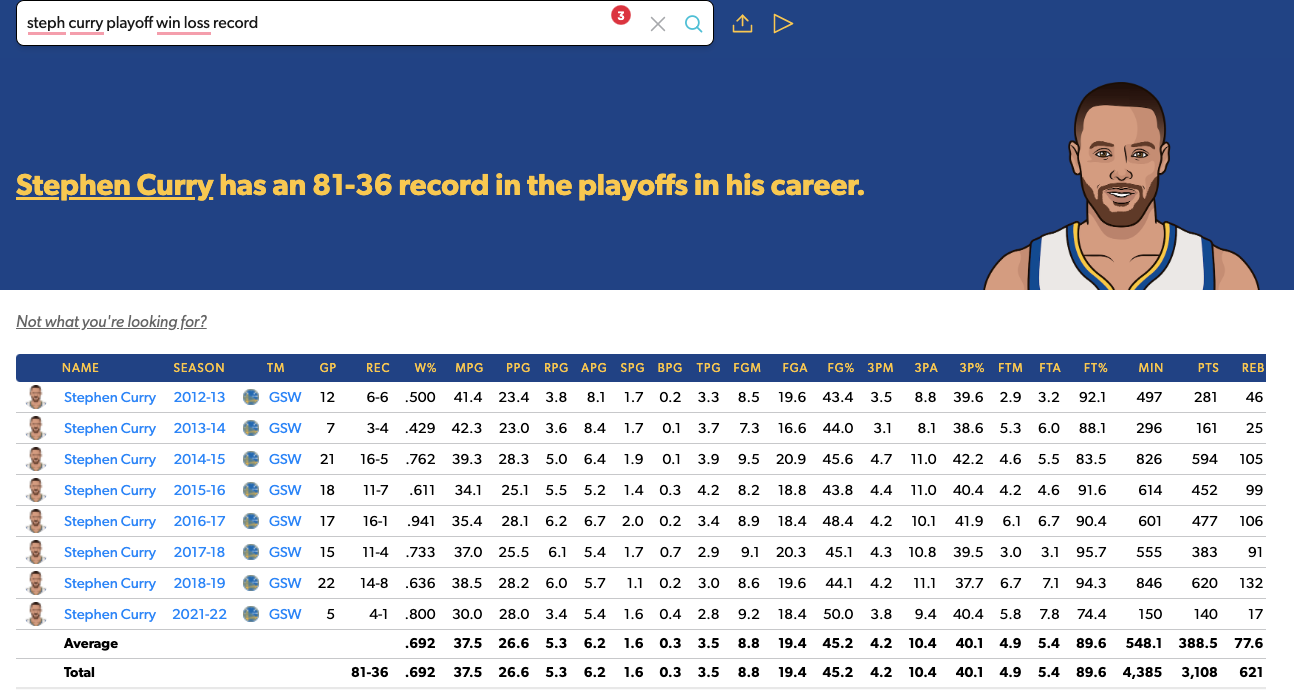
\includegraphics[width=.98\linewidth]{StatsMuse_Curry.png}
    \caption{
        Steph Curry's Playoff W/L Record with Stats
    }
    \label{fig:second-page-2}
\end{figure}

\section{Methods}

What I plan on doing for collecting the NBA stats for my project would be to query them from sports stats database like SportsReference. I would have to make an algorithm to pull these stats from the website based on what player the user chooses like "Stephen Curry" or "Lebron James" and what stats they specifically choose to evaluate the players and make comparisons.

For how the statistical data is going to be calculated and shown on a graph/chart, I need to create an algorithm using python to create and display data on a graph and show the stats used on a chart below. A mathematical model would need to be used for the data/stats and how to calculate them to make them used as a value for the player's value.

The data I am going to show is what players the project recommends to the fantasy users based on the stats they choose to compare the players. They will use this information to influence their draft picks and evaluate the player value. This graph produced shows the user players that are statistically similar to the player of their choosing and the stats that they also want to compare. The data shown would be a graph with different points of data that represents a player in the NBA and below the graph would be a chart of the data to see what was used to calculate the graph's data points. The graph's data will be calculated using the stats chosen by the user and will be plotted with reference to where the player is based on those stats. For example, if the user picks 3 pointer made, field goals made and assists as the data to be compared, it will show the user a graph of the player chosen like Ja Morant compared to other player with stats that are similar and create many points of data on the graph. It will look roughly like Figure 2, but the graph is more simplistic and gives information for what point of data represent a certain player and shows the chart of data used to compare. 

Obtaining the data for this project would require Python being used and querying sports websites for the stats like \url{basketballreference.com} and \url{stats.nba.com}. I would extract the statistical data from the previous regular season, so 2021-22 season, and then add the data to a csv file. From there I can query the data that the user chooses, for example total points and rebounds, and then have a data sheet of players and those specific stats. Then, the algorithm would look at the stats in the data sheet and calculate points of data on the graph and set the points with the player chosen highlighted. When a user drags the mouse over a point of data, it says the name of the player

Datasets of surveys of people who might want to use my app for fantasy to look for the value of players will be useful for my project methods because of what they would want the user interface to have to make it easy to evaluate the data. I would talk to fantasy basketball users and discuss what they are looking for when drafting players for their fantasy team. I would ask them what stats they look for when picking players, what positions they prioritize in fantasy and how they would use data given to them based on looking at a visualization of sports statistics. I would ask them about their strategies of drafting players and if they do it based on personal opinions about the player, like wanting a "star" in the NBA or statistical data, which can be underrated players. To do a mock fantasy draft as a way to test the potential of the project would be to make the fantasy users pick a player from each position that they like and use the project to do the comparisons of stats for each of those players. They would write down 5 other NBA players that are statically similar in a chart under those players just in case they get chosen in the draft and have backup options. While doing a mock fantasy draft, the users can see if they can get the players that they wrote down and simulate a season for fantasy to see if the players chosen performed to their expectations based on the project. I would get feedback from the users to see what their opinion was on draft certain players that they picked from the graph of the project.  


\section{Evaluation}

For this summer to evaluate my project, I would do mock fantasy drafts and simulate the fantasy seasons based on the 2021-22 season to see results using my project to pick players. My project would be used to find a player with the specific stats that the user wants to take advantage of when other similar players are taken off the board like a superstar in the NBA like Lebron James. The fantasy season would be simulated to see what place the user got in fantasy and to see if the players that were recommended had a positive impact on their team. The list of players that the user produced from the project would be used to influence how the user drafts players in the mock draft. Since they will have many options for each position that the player user has to fill for their team, they can find players that were statistically similar to the player that they like or are considered a "star" in the league. Results from a simulated fantasy season will allow the user to see the impact of the players chosen from the project based on how many individual fantasy points were scored. I would get feedback from the users to see if they agreed with what the project produced when they used it and if they thought the project was accurate in evaluating the players. It would be based on the user's opinion because NBA players picked in fantasy drafts can under perform and user's would not like that because of how there will be a lack of fantasy points. I will ask them if the visualization was easy to follow and comprehend when evaluating the player and other players statically. I would ask if looking at the chart of the stats were more effective than looking at the visualization on the graph and vice versa. Another question would be if the project worked well both with the visualization and the chart for reference or if one was better than the other at evaluating players. Asking the user what statistics they prioritize in fantasy is key because fantasy sports is all about scoring fantasy points and not losing points based on specific stats like turnovers and fouls. 

A source I would use to evaluate the player chosen in the draft would be using the Yahoo Fantasy Draft Analysis \cite{fantasy}. This website shows you data of the average pick that users picked the player, what average round they were selected and the percent drafted in all Yahoo fantasy sports leagues. These statistics are used to see how popular draft picks are and with it, you can click on the player and it will show the NBA stats and fantasy stats points and the ranking of the player. The user can use this website to evaluate the players they chose and can give feedback whether it was a good pick, neutral pick or bad pick. They will give feedback on if they thought the project misdirected them or helped them with their picks. Figure 4 show the top 5 players picked in fantasy sports for the 2021-22 NBA season. The highlighted blue box column allows a user to look at the fantasy sports statistics and see the rankings of the players for the year.

\begin{figure}
    \centering
    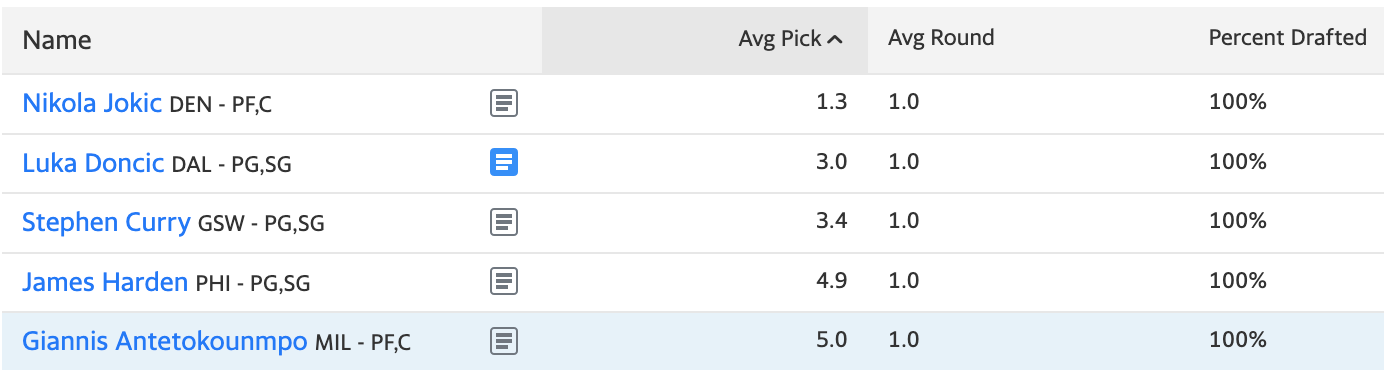
\includegraphics[width=.98\linewidth]{top5.png}
    \caption{
        Yahoo Fantasy Draft Analysis Top 5 Picks 2021-22 Season
    }
    \label{fig:second-page-4}
\end{figure}

Another source that I can use for evaluation is the ESPN mock draft website \cite{fantasyDraft}. This would allow a user to test the project by doing mock drafts and seeing what players they can pick for their team. Using my project would help influence the users to pick players that are statistically similar to a player that was already chosen. Then the user can join a fantasy league and simulate the previous basketball season to see how well the team performed with the players based off the project. To be able to evaluate how well the project worked, I would ask them if drafting the players were positive or negative based on what the graph produced when comparing NBA players and their stats. A question would be what kind of stats they compared and if they would change them if something did not work out. I would also ask them what kinds of fantasy league it is like head-to-head, most points overall, or categories of stats and which one type of league would best benefit from using the project. For this draft simulation, I would ask the users what strategies they use for fantasy drafts in general and what they would do differently using my project for influencing their decisions. Figure 5 shows what kinds of mock drafts a fantasy player can do with different league rules of how scoring it tallied, which can change how the project is evaluated. If the users can spot differences in choosing players in different types of fantasy leagues, I can evaluate which fantasy league would be the best option to use my project for

\begin{figure}
    \centering
    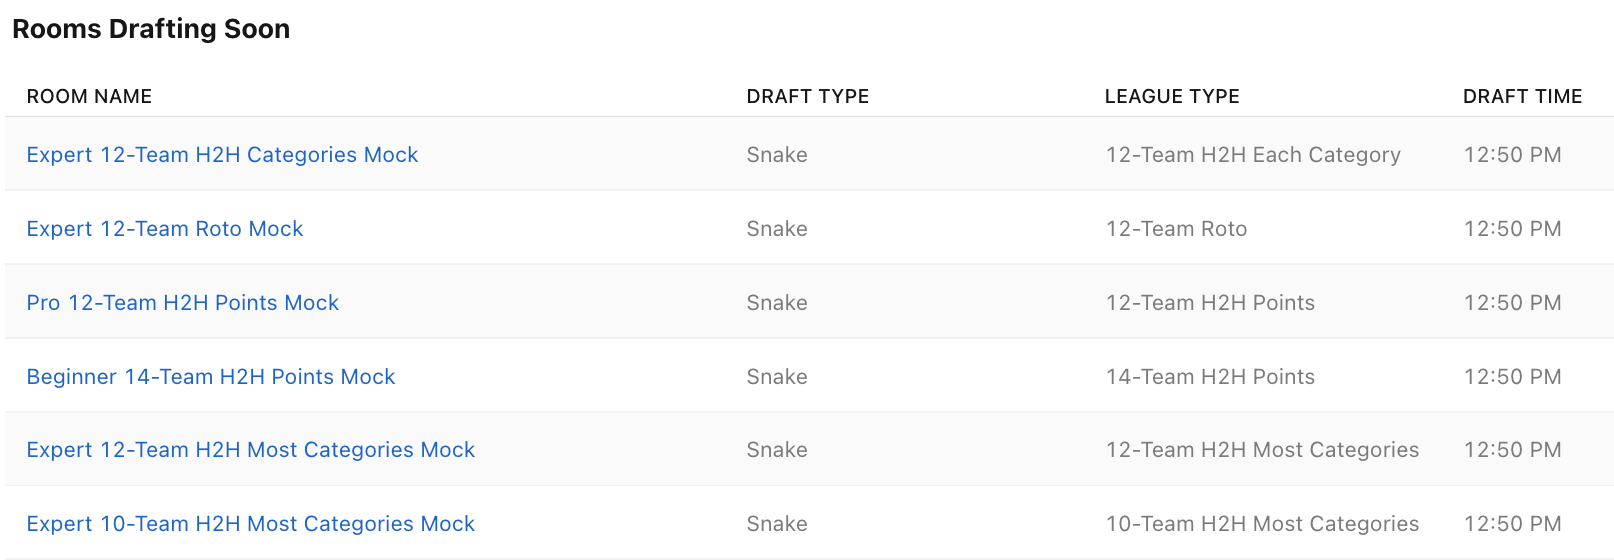
\includegraphics[width=.98\linewidth]{mockdraft.png}
    \caption{
        Different Types of Fantasy League for Mock Draft
    }
    \label{fig:second-page-5}
\end{figure}

Overall, I will gather all the information I received to evaluate how well my project would influence a fantasy player to use it to help draft a team. Evaluating the reactions of using my project from the user standpoint is a big say to see if the project positively or negatively helped their team or if they thought the project was useful or not. I can calculate different variables of percent of users satisfied using the project, if the team did well in fantasy and if the players chosen were a good choice overall. I can also calculate the percent of users satisfied with the project itself and using it to compare players and take the feedback to improve the project and pin point issues with using it. 

\section{Ethical Considerations}
Some ethical concern with my project might be how money is involved in fantasy sports and my project can influence people to bet and potentially lose money if they use my project's outcome to draft players. If a users is deadset on just using my project and influenced them to bet much of their money on thinking my project will get them a guaranteed win, it can be unethical because that is not what my project is for and it is only to help a user evaluate players to potentially draft in fantasy.  


\section{Timeline}
For the timeline of my project starting this summer, I have to start thinking about programming the project for my testing users. Below is a list of all the dates for my project and major events that need to happen to fulfill finishing my project on time. 

\begin{itemize}
    \item 5/15: Think about how to program pulling stats from websites
    \item 5/30: Think about how to code graphs using python
    \item 6/14: Start coding
    \item 6/30: Start coding
    \item 7/14: 
    \item 7/30:
    \item 8/14: 
    \item 8/30: 
    \item 9/14:
    \item 9/30:
    \item 10/14:
    \item 10/30:
    \item 11/14: Finish poster
    \item 12/5 Poster presentations
    \item 12/15 Final paper and code due
\end{itemize}


\printbibliography 

\end{document}